\documentclass[12pt, a4paper]{article}

\usepackage[utf8]{inputenc}
\usepackage[spanish]{babel}
\usepackage{titling}
\usepackage[left=2cm,right=2cm,top=2cm,bottom=2cm]{geometry}
\usepackage{enumerate}
\usepackage{amsmath}
\usepackage{graphicx}
\usepackage{caption}
\usepackage{float}

\usepackage{listings}%-para agregar codigo-
\usepackage[usenames,dvipsnames]{color}
\usepackage{color}%------------------------

%---------------------importar codigo desde archivos cpp----------------------------
\lstloadlanguages{C++}
\lstnewenvironment{code}
	{%\lstset{	numbers=none, frame=lines, basicstyle=\small\ttfamily, }%
	 \csname lst@SetFirstLabel\endcsname}
	{\csname lst@SaveFirstLabel\endcsname}
\lstset{% general command to set parameter(s)
	language=C++, basicstyle=\small\ttfamily, keywordstyle=\slshape,
	emph=[1]{tipo,usa}, emphstyle={[1]\sffamily\bfseries},
	morekeywords={tint,forn,forsn},
	basewidth={0.47em,0.40em},
	columns=fixed, fontadjust, resetmargins, xrightmargin=5pt, xleftmargin=15pt,
	flexiblecolumns=false, tabsize=2, breaklines,	breakatwhitespace=false, extendedchars=true,
	numbers=left, numberstyle=\tiny, stepnumber=1, numbersep=9pt,
	frame=l, framesep=3pt,
    basicstyle=\ttfamily,
    keywordstyle=\color{blue}\ttfamily,
    stringstyle=\color{magenta}\ttfamily,
    commentstyle=\color{RedOrange}\ttfamily,
    morecomment=[l][\color{OliveGreen}]{\#}
}

\lstdefinestyle{C++}{
	language=C++, basicstyle=\small\ttfamily, keywordstyle=\slshape,
	emph=[1]{tipo,usa,tipo2}, emphstyle={[1]\sffamily\bfseries},
	morekeywords={tint,forn,forsn},
	basewidth={0.47em,0.40em},
	columns=fixed, fontadjust, resetmargins, xrightmargin=5pt, xleftmargin=15pt,
	flexiblecolumns=false, tabsize=2, breaklines,	breakatwhitespace=false, extendedchars=true,
	numbers=left, numberstyle=\tiny, stepnumber=1, numbersep=9pt,
	frame=l, framesep=3pt,
    basicstyle=\ttfamily,
    keywordstyle=\color{blue}\ttfamily,
    stringstyle=\color{magenta}\ttfamily,
    commentstyle=\color{RedOrange}\ttfamily,
    morecomment=[l][\color{OliveGreen}]{\#}
}

\def\nbtitle#1{\begin{Large}\begin{center}\textbf{#1}\end{center}\end{Large}}
\def\nbsection#1{\section{#1}}
\def\nbsubsection#1{\subsection{#1}}
\def\nbcoment#1{\begin{small}\textbf{#1}\end{small}}
\newcommand{\comb}[2]{\left( \begin{array}{c} #1 \\ #2 \end{array}\right)}
\def\complexity#1{\texorpdfstring{$\mathcal{O}(#1)$}{O(#1)}}
 \newcommand\cppfile[2][]{
\lstinputlisting[style=C++,linerange={#1}]{#2}
}
%%------------------------------------------------------------------------------

\newcommand{\subtitulo}[1]{\begin{center}\textbf{#1}\end{center}}

\title{\textbf{Programación Dinámica}}
\author{Wilmer Emiro Castrillón Calderón}

\graphicspath{{../}}
\newcommand*\lstinputpath[1]{\lstset{inputpath=#1}}
\lstinputpath{../}

\begin{document}
	\maketitle
	
	%<*Capitulo>
	
	\section{Introducción a la programación dinámica}
	\label{dp:introduccion}
	
	La programación dinámica es una metodología utilizada para reducir la complejidad computacional a un
	algoritmo, es usada principalmente para resolver problemas de optimización y conteo,
	se basa en la estrategia \textit{divide y vencerás}, consiste en tomar un problema complejo y dividirlo 
	sucesivamente en subproblemas mas pequeños hasta llegar a un caso base, y partir de ahí empezar a construir la
	solución de cada subproblema, hasta llegar a una solución global. Durante la búsqueda de soluciones
	se utiliza tablas de memorización, en la cuales se guarda la solución óptima de cada subproblema.
	Como abreviatura a programación dinámica se suele utilizar \textit{dp}, pues son sus siglas en ingles.\\
	
	Los problemas de programación dinámica presentan tres condiciones básicas:
	\begin{enumerate}[1.]
		\item El problema se puede dividir en subproblemas, y estos a su vez en más subproblemas, y así hasta llegar
				a uno o múltiples casos base.
		\item La solución óptima de cada subproblema depende de la solución óptima de cada uno de sus
				propios subproblemas, entonces cumple con el principio de optimalidad de Bellman.
		\item Se presenta superposición de problemas, es decir, existen sub-problemas que aparecen múltiples veces
		 		a lo largo de la búsqueda de la solución general. Esta es la razón principal que le permite tener menor  
				complejidad computacional.
	\end{enumerate}
	
	\subtitulo{Ejemplo inicial.}
	
	Como un ejemplo básico se puede utilizar la sucesión de Fibonacci, esta comienza con los números 0 y 1, y a partir
	de estos dos números iniciales los siguientes son la suma de los dos anteriores, entonces los primeros
	números de Fibonacci son los siguientes:
	\begin{center} $0, 1, 1, 2, 3, 5, 8, 13, 21, 34, 55, 89, ..... $ \end{center}
	
	Ahora se buscará resolver el siguiente problema: dado un numero $i$ calcular el $i$-esimo numero de Fibonacci. 
	Para dar una solución con dp se deben identificar los subproblemas, y la solución a cada subproblema se debe  
	guardar en una tabla de memorización. En este caso la tabla de memorización será un vector $v$ en el cual la  
	posición $i$-esima del vector corresponderá al número $i$-esimo de la sucesión, y para la división en subproblemas  
	se puede escribir la siguiente formula recursiva:\\
	\begin{center}
		$fibo(n) = 	
			\begin{cases}
				n & \text{if $n\le 1$}\\
				fibo(n-1) + fibo(n-2) & \text{if $n\ge 2$}
		\end{cases}	$\\
	\end{center}
	
	Para implementar dp surgen dos enfoques: Top-Down y Buttom-Up.\\
	
	\textbf{Buttom-Up}\\
	En este enfoque se irá recorriendo la tabla de memorización mientras se llena, se comienza con los
	casos base de la formula recursiva y a partir de ahí se deberá calcular y guardar los demás resultados. En este  
	enfoque primero se calcula el resultado de todos los subproblemas antes de dar alguna solución global. Aunque   
	este enfoque sea iterativo puede resultar mas difícil de implementar, pues por lo general es menos intuitivo.\\
	
	Para este ejercicio comenzamos llenando en un vector $v$ los casos base: $v[0] = 0$ y  $v[1] = 1$, después 
	se llena el resto del vector según se indica en la formula recursiva: $v[i] = v[i-1] + v[i-2]$, de tal forma que  
	$v[i-1]$ y $v[i-2]$ son valores que se han calculado antes y ademas $v[x] = fibo(x)$. A continuación se muestra el  
	ejemplo en C++ calculando los primero $45$ números de la sucesión:
	\cppfile[7-12]{Programacion_dinamica/codigos/fibo.cpp}
	
	\textbf{Top-Down}\\
	A diferencia del anterior enfoque en este se utilizan llamados recursivos, en los cuales se irá guardando
	los resultados en la tabla de memorización mientras se calculan, y así evitar que se realice dos veces el
	mismo llamado recursivo. En este enfoque se hace mas notorio la importancia de la tabla de memorización, si se  
	escribiera únicamente la formula recursiva, como se muestra en el código de abajo, se obtendría una solución 
	ineficiente, pues para $fibo(6)$ se obtendría el árbol de recursión de la figura 
	\ref{dp:introduccion:arbol_recursion}.
	\cppfile[14-19]{Programacion_dinamica/codigos/fibo.cpp}

	\begin{figure}[!htb]
		\centering
		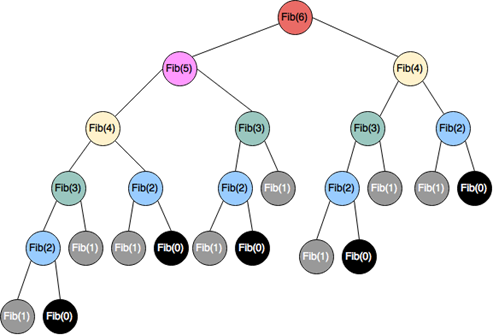
\includegraphics[scale=0.9]{Programacion_dinamica/imagenes/introduccion/arbol_recursion}
		\caption{}
		\label{dp:introduccion:arbol_recursion}
	\end{figure}
	
	Se puede observar en la figura \ref{dp:introduccion:arbol_recursion} que se realizan múltiples 
	llamados repetidos, $fibo(4)$ se repite 2 veces, $fibo(3)$ 3 veces, $fibo(2)$ 5 veces, $fibo(1)$ 8 veces y 
	$fibo(0)$ 5 veces, resultan bastantes llamados recursivos solamente para encontrar $fibo(6)$, esta solución tiene 
	una complejidad exponencial, en números pequeños no es muy notorio pero cuando intentamos encontrar $fibo(45)$ el 
	tiempo de ejecución se hace muy alto, entonces para mejorar el tiempo se debe implementar una tabla de  
	memorización, en la cual se guarde el resultado de cada llamado recursivo, ademas se debe agregar un condicional al 
	inicio del método para validar si la solución de ese subproblema ya fue encontrada, en tal caso se devuelve el  
	valor guardado, sino se calcula y se guarda, en este ejemplo la tabla comienza llena con -1, un valor que nunca es  
	usado en la solución, de tal forma que si una posición es igual a -1 entonces se debe calcular.
	
	\begin{minipage}{\linewidth}
		\cppfile[24-31]{Programacion_dinamica/codigos/fibo.cpp}
	\end{minipage}
	
	Este ejercicio resulta muy trivial, se puede resolver fácilmente sin pensar en dp, ahora se mostrara otro
	problema en el cual se hace necesario utilizar dp para dar una solución eficiente.
	
	\subtitulo{Recorrido óptimo en una matriz.}
	
	Teniendo una matriz de $n$ x $m$ con números enteros, se quiere conocer la suma máxima que se puede obtener
	recorriendo la matriz, comenzando desde la esquina superior-izquierda y terminando en la esquina inferior-derecha,
	realizando únicamente pasos hacia la derecha y abajo, por ejemplo:\\
	\begin{table}[h]
		\centering
		\begin{tabular}{|l|l|l|}
			\hline
			5  &6 &4 \\ \hline
			3  &8  &5 \\ \hline
			2 &11 &15 \\ \hline
			5 &2  &17 \\ \hline
		\end{tabular}
		\caption{}
		\label{dp:introduccion:recorrido_matriz1}
	\end{table}
	
	El camino óptimo es 5-6-8-11-15-17 y la suma es 62. Este es un problema de optimización, a simple vista la solución 
	consistiría de siempre ir a la casilla adyacente con mayor valor, pero no siempre es el mejor camino, por ejemplo  
	con la siguiente matriz:
	\begin{table}[H]
		\centering
		\begin{tabular}{|l|l|l|l|}
		 	\hline
			1  & 12 & 4  & 9 \\ \hline
			6  & 5  & 21 & 15 \\ \hline
			35 & 18 & 8  & 10 \\ \hline
			12 & 2  & 4  & 15 \\ \hline
		\end{tabular}
		\caption{}
		\label{dp:introduccion:recorrido_matriz_2}
	\end{table}
	
	No es una solución óptima ir a la siguiente casilla con mayor valor, pues haciendo esto se tendría el siguiente
	camino 1-12-5-21-15-10-15 con un acumulado de 79, en cambio el camino 1-6-35-18-8-10-15 tiene un acumulado de 93,
	entonces con la anterior estrategia no siempre se obtiene el camino óptimo. En este problema es necesario realizar
	una toma de decisiones, pues existen múltiples opciones de caminos, y se necesita encontrar el conjunto de
	decisiones que permita llegar a un resultado optimo, una solución inicial puede ser con BackTraking pero esta 
	tendría complejidad exponencial O($2^{n}$), por lo tanto se necesita utilizar otro enfoque.\\
	
	Este problema se puede resolver con programación dinámica, pues se puede encontrar la solución general a partir de 
	la solución de sub-problemas más pequeños, supongamos que tenemos una matriz $T$ de tamaño $n$ x $m$, para  
	encontrar el camino óptimo hasta $T[n-1][m-1]$(ultima casilla) es necesario primero 
	encontrar el óptimo de $T[n-2][m-1]$ y $T[n-1][m-2]$, pues para llegar a $T[n-1][m-1]$ hay dos opciones, llegar 
	por arriba (equivalente a tomar la decisión ir-abajo desde $T[n-2][m-1]$) o llegar por la izquierda (equivalente 
	a tomar la decisión ir-derecha desde $T[n-1][m-2]$), entonces la solución general sera \textit{T[n-1][m-1] + 
	máximo(camino óptimo hasta T[n-2][m-1], camino óptimo hasta T[n-1][m-2])}, y a su vez el óptimo para $T[n-2][m-1]$ 
	y $T[n-1][m-2]$ se calcula de manera similar, de esta forma se puede dividir el problema general en subproblemas.\\
	
	La solución general se puede escribir como una formula recursiva $f(i,j)$ la cual devolverá el valor del recorrido 
	optimo desde $T[0][0]$ hasta $T[i][j]$, donde $i$ es la posición de fila y $j$ la posición de columna, si $i$ y 
	$j$ son iguales a $0$ entonces el resultado es $T[0][0]$(se encuentra en el punto inicial), si solo $i$ es $0$ 
	entonces el resultado es $T[0][j] + f(0,j-1)$, solo se puede llegar a $T[0][j]$ desde su izquierda, pues desde 
	arriba estaría afuera de la matriz, si solo $j$ es $0$ entonces de manera similar se tiene como resultado 
	$T[i][0] + f(i-1,0)$, con base en esto se puede construir la siguiente formula recursiva:
	\begin{center}
		$f(i, j) = 	
		\begin{cases}
			T[0][0] & \text{if $i,j = 0$}\\
			T[0][j] + f(0, j-1) & \text{if $i = 0$}\\
			T[i][0] + f(i-1, 0) & \text{if $j = 0$}\\
			T[i][j] + max(f(i-1, j), f(i, j-1)) & \text{if $i,j \neq 1$}
		\end{cases}
	$\\
	\end{center}
	Realizando manualmente la función recursiva se puede tener mas claridad. El caso $f(0,0)$ indica que la solución
	es el elemento en $T[0][0]$, la solución para la primera fila sera la sumatoria de los elementos desde 
	la primera casilla hasta la columna correspondiente, ese es el único camino posible, de similar manera ocurre
	con la primera columna (figura \ref{dp:introduccion:matriz1}), para los demás casos se abren dos opciones, llegar  
	desde arriba o llegar desde la izquierda (figura \ref{dp:introduccion:matriz2}), la formula indica tomar el de 
	mayor valor, de esta manera mientras se avanza se ira seleccionando el mejor camino hasta llegar a la ultima 
	casilla (figura \ref{dp:introduccion:matriz3}).\\
	
	\begin{figure}[!htb]
		\minipage{0.33\textwidth}
			\centering
			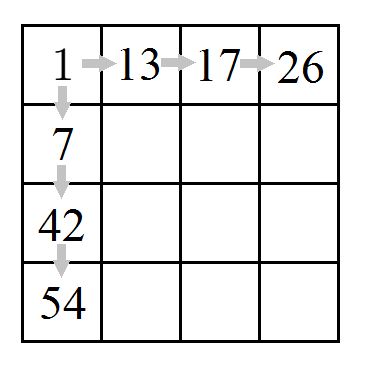
\includegraphics[scale=0.4]{Programacion_dinamica/imagenes/introduccion/matriz1}
			\caption{}
			\label{dp:introduccion:matriz1}
		\endminipage
		\minipage{0.33\textwidth}
			\centering
			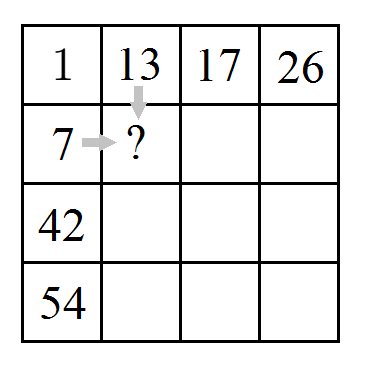
\includegraphics[scale=0.4]{Programacion_dinamica/imagenes/introduccion/matriz2}
			\caption{}
			\label{dp:introduccion:matriz2}
		\endminipage
		\minipage{0.33\textwidth}
			\centering
			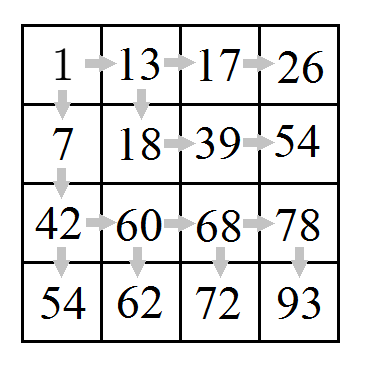
\includegraphics[scale=0.4]{Programacion_dinamica/imagenes/introduccion/matriz3}
			\caption{}
			\label{dp:introduccion:matriz3}
		\endminipage
	\end{figure}
	
	Para terminar el dp es necesario agregar la tabla de memorización, pues aplicar la formula directamente resultaría 
	en un algoritmo de complejidad exponencial, como tabla de memorización se usara otra matriz de igual tamaño, en  
	este ejemplo se llamara $memo$ y guardara las soluciones, es decir, que en $memo[i][j]$ se guarda el acumulado 
	óptimo para ir desde $T[0][0]$ hasta $T[i][j]$, ahora se puede solucionar el problema usando cualquiera de los dos 
	enfoques de dp. La complejidad algorítmica resultante para ambos enfoques es O($n*m$), resultando mucho mejor que 
	un algoritmo de complejidad exponencial utilizando fuerza bruta.\\
	
	Para usar Top-Down solamente se agrega la tabla de memorización a la formula recursiva, y se verifica si la 
	solución al subproblema ya fue encontrada. Para obtener el resultado se debe invocar $f(n-1, m-1)$. La 
	implementación es la siguiente:
	\cppfile[9-17]{Programacion_dinamica/codigos/matriz.cpp}
	
	Para la solución con Buttom-Up se debe recorrer la matriz y llenarla según la formula recursiva, se debe comenzar  
	con los casos base antes de calcular lo demás. De esta forma para conocer la solución se debe imprimir 
	$memo[n-1][m-1]$. La implementación es la siguiente:
	\cppfile[19-31]{Programacion_dinamica/codigos/matriz.cpp}
		
	\section{Sub-SetSum}
	\label{dp:sub_set_sum}
	
	También conocido como suma de subconjuntos, el problema consiste en que dado un conjunto de números enteros
	$V$, encontrar si es posible que un número $n$ sea el resultado de la suma de los elementos de algún
	subconjunto de $V$, por ejemplo con el conjunto $V$={1, 2, 5} es posible sumar 7 usando el subconjunto \{2, 5\},
	con este conjunto $V$ seria posible sumar \{1, 2, 3, 5, 6, 7, 8\}.\\
	
	Este es un problema de decisión, para cada elemento en $V$ existen dos posibilidades, tomarlo o no, y	validar 
	si el subconjunto de elementos seleccionados suman $n$, un algoritmo de BackTraking tiene una complejidad 
	O($2^{n}$) para cada consulta, es decir, si se necesita validar $Q$ números distintos el proceso se repite $Q$  
	veces, una mejor opción es calcular todos los posibles subconjuntos y guardar todas las posibles soluciones, esto
	implica un precalculo con complejidad O($2^{n}$) que es muy alto pero permite responder cada consulta en  
	complejidad constante.\\
	
	Este problema puede ser resuelto de manera mas eficiente usando dp, se puede
	reescribir el numero $n$ como: $n=V[k_{1}]+x_{1}$, con $V[k_{1}]$ como algún numero en $V$, de manera similar se
	puede reescribir $x_{1}$ como $x_{1}=v[k_{2}]+x_{2}$ y así sucesivamente hasta encontrar $x_{n}=v[k_{n}]+0$, de 
	esta manera si se toma cada elemento de $V$ que fue utilizado, se podría encontrar el subconjunto 
	$\{v[k_{1}],v[k_{2}],...,v[k_{n}]\}$ el cual sumando todos sus elementos obtenemos $n$.\\
	
	En este problema el resultado deberá ser 'verdadero' o 'falso', mostrando si es posible sumar $n$ con algún 
	subconjunto, con los subproblemas establecidos se puede ahora definir los casos base, si en algún momento 
	se llega a $x_{n}=0$ entonces la solución global sera 'verdadero'(se encontró una solución, entonces es posible 
	sumar $n$), pero si en algún momento usamos todos los elementos en $V$ y aun $x_{n}>0$, o 
	en algún momento se llega a $x_{n}<0$ entonces la solución en ese subproblema sera 'falso', entonces se tiene la
	siguiente función recursiva:
	\begin{center}
		$f(n, k) = 	
		\begin{cases}
			1 & \text{if n = 0}\\
			0 & \text{if n $<$ 0, k$>longitud($V$)$}\\
			1 & \text{if $f(n-V[k],k+1)=1$ o $f(n,k+1)=1$}\\
			0 & \text{if $otro$}
		\end{cases}
		$\\
	\end{center}
	Con esta formula la solución sera igual a $f(n,0)$, para implementarla se debe hacer una tabla de memorización,
	la cantidad de columnas de la tabla debe ser por lo menos igual a la longitud del vector, y la cantidad 
	de filas por lo menos igual al resultado más grande que se puede obtener, y como valor inicial se puede usar $-1$.
	\cppfile[24-33]{Programacion_dinamica/codigos/SubSetSum.cpp}
	
	Otra posible solución al problema es utilizando el enfoque Buttom-Up, los subproblemas se podrían ver de la  
	siguiente manera, tomando a $m$ con el tamaño del vector $V$, la solución general incluye sumar el
	elemento $V[m-1]$ a todas las posibles sumas encontradas hasta $V[m-2]$, y este a su vez depende de encontrar las
	sumas hasta $V[m-3]$ y así sucesivamente hasta llegar a $V[0]$ que es el caso base, mas detalladamente la  
	solución hasta $V[0]$ es solamente él mismo, las posibles sumas hasta $V[1]$ es el conjunto 
	\{$V[0]$, $V[1]$, $V[0]+V[1]$\}, ahora las posibles sumas hasta $V[2]$ son 
	\{$V[0]$, $V[1]$, $V[2]$, $V[0]+V[1]$, $V[0]+V[2]$, $V[1]+V[2]$, $V[0]+V[1]+V[2]$\}, y así sucesivamente hasta  
	llegar a $V[m-1]$, descartando números repetidos.\\
	
	Por ejemplo sea $V$=\{3, 5 y 8\}, comenzando con $V[0]$ el conjunto de soluciones es \{3\}, tomando el elemento
	$V[1]$ el conjunto de soluciones pasa a ser a \{3, 5, 8\}, y por ultimo incluyendo $V[2]$ el conjunto resultante  
	es: \{3, 5, 8, 11, 13, 16\}. Una posible implementación es la siguiente:\\
	\cppfile[8-21]{Programacion_dinamica/codigos/SubSetSum.cpp}
	
	En el anterior código se tienen dos ciclos, el primero recorriendo el vector $V$ y el segundo buscando las 
	soluciones anteriores para sumarles $V[i]$, como el caso base es cuando $i=0$ entonces se debe omitir el segundo
	ciclo cuando $i$ tiene este valor, ejecutando este código se obtendría todas las soluciones en la última columna,
	entonces si $memo[n][V.size()-1]$ es verdadero entonce si existe un sub-conjunto que sume $n$, en caso contrario
	no es posible.

	\section{Problema de la mochila(Knapsack problem)}
	\label{dp:problema_de_la_mochila}
	
	Este es un problema clásico de programación dinámica, consiste en lo siguiente, hay una mochila que tiene una
	capacidad limitada de peso que puede contener, y hay un grupo de objetos, cada uno tiene un valor y peso, el
	objetivo consiste en llenar la mochila con los objetos de tal forma que no se exceda su capacidad de peso y 
	que el valor de los objetos que hay dentro de la mochila sea lo más alto posible. Por ejemplo:
	\begin{center}
		\begin{tabular}{|l|l|l|l|l|l|l|}
			\hline
			$i$  	&0 &1 &2 &3 &4 &5 \\ \hline
			$W_{i}$ &1 &2 &4 &5 &4 &2 \\ \hline
			$V_{i}$ &2 &7 &5 &9 &5 &3 \\ \hline
		\end{tabular}
	\end{center}
	Sea $N=6$ la cantidad de objetos, $C=10$ la capacidad de la mochila, $W_{i}$ el peso del i-ésimo objeto y 
	$V_{i}$ el valor del i-ésimo objeto, entonces las respuesta es 21, usando los objetos 0, 1, 3, 5 obtenemos un peso 
	10 con valor 21.\\
	
	Para cada objeto existen dos opciones, tomarlo o dejarlo, entonces para n objetos existen $2^{n}$ posibles 
	opciones, de todas ellas la solución será una configuración que no exceda el peso de la mochila y la suma de los
	objetos seleccionados sea el más alto, una solución probando todos los posibles casos tendrá complejidad 
	O($2^{n}$), la cual es bastante alta, mientras que una solución greddy no siempre va a funcionar.\\

	Sin embargo es posible reducir bastante la complejidad trabajando con programación dinámica, sea $x_{i}$ la 
	capacidad usada al estar en el i-ésimo objeto, iniciando con $i=0$ y $x_{i}=0$, se repite el siguiente proceso: 
	para cada objeto existe la decisión de no tomarlo y pasar al objeto $i+1$ con $x_{i+1}=x_{i}$ o tomarlo y pasar 
	al objeto $i+1$ con $x_{i+1}=x_{i}+W_{i}$ siempre y cuando $x_{i}+W_{i} \leq C$, es decir que no se exceda la 
	capacidad, entonces se puede escribir la siguiente función recursiva:
	\begin{center}
		$f(i, x) = 	
		\begin{cases}
			0 & \text{if } i = N\\
			max(f(i+1,x), f(i+1,x+W_{i}) + V_{i}) & \text{if } x+W_{i} \leq C \\
			f(i+1,x) & \text{if $otro$}
		\end{cases}
		$\\
	\end{center}
	
	Al programar esta función recursiva se obtendrá una complejidad de $O(2^{n})$, pero al agregar la tabla de 
	memorización la complejidad se reduce al tamaño de la tabla, quedado en $O(N*C)$, y finalmente se puede obtener 
	la siguiente implementación.
	\cppfile[9-17]{Programacion_dinamica/codigos/ProblemaMochila.cpp}
	
	\section{Traveling salesman problem}
	\label{dp:TSP}
	
	El problema del vendedor viajero o \textit{Traveling salesman problem} en ingles, es un problema clásico el cual 
	consiste en lo siguiente: Un vendedor quiere visitar $n$ ciudades comenzando desde una ciudad cualquiera y al 
	finalizar regresar a la ciudad inicial, ¿cual es la ruta mas corta posible?. Este problema consiste en encontrar
	el ciclo hamiltoniano mas corto en un grafo, la principal dificultad es la cantidad de posibles rutas, pues la 
	cantidad de posibles caminos puede llegar hasta $n!$. Este es un problema clásico que ha sido estudiado por 
	décadas y una de sus mejores soluciones es utilizando programación dinámica. Por ejemplo en la figura 
	\ref{dp:TSP:ejemplo} la respuesta optima es $35$ siguiendo el camino $2,4,3,1,5,0,2$.\\
	
	\begin{figure}[!htb]
		\centering
		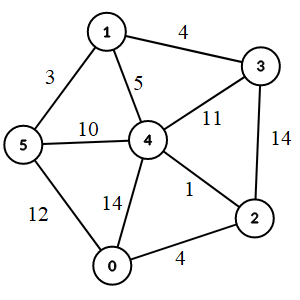
\includegraphics[scale=0.9]{Programacion_dinamica/imagenes/TSP/ejemplo}
		\caption{}
		\label{dp:TSP:ejemplo}
	\end{figure}
	
	En grafos completos(grafos en los cuales existen aristas conectando todos los posibles pares de aristas) 
	la cantidad total de posibles rutas es $n!$ lo cual hace que un algoritmo de backtraking solo se pueda aplicar
	para grafos muy pequeños, de menos de 12 aristas. Una mejor solución es utilizando programación dinámica con
	mascara de bits, en esta mascara se van a marcar como visitados los nodos de tal forma que si el $i$-esimo bit 
	de la mascara es $1$ entonces el nodo $i$ ya esta visitado, si es $0$ entonces esta disponible, la idea general  
	consiste en ir tomando nodos disponibles e ir sumando la distancias entre el ultimo par de nodos seleccionados, 
	como se puede observar en la siguiente formula recursiva.
	
	\begin{center}
		$f(m, v) = 	
		\begin{cases}
			dist(v, 0) & \text{if } m = 2^{n}-1\\
			min(f(m|(2^{i}), i) + dist(v, i)) & \text{if $otro$}
		\end{cases}
		$\\
	\end{center}
	
	Para la implementación se utiliza una tabla de memorización de tamaño $2^{n}$ x $n$, también se necesita una
	matriz de adyacencia para obtener rápidamente la distancia entre cualquier par de nodos, como la ruta es un ciclo 
	el primer nodo también debe ser el ultimo, entonces se puede iniciar en cualquier nodo y al recorrer todos los  
	demás se debe volver al nodo inicial, lo mas sencillo es dejar el primer nodo como el primero y ultimo.\\
	
	En cada llamado recursivo se deben recorrer los $n$ bits de la mascara buscando los nodos disponibles, 
	para cada uno de ellos se debe hacer un llamado recursivo tomando ese nodo como el siguiente de la ruta, al final 
	se debe tomar el valor que minimice el acumulado total, el caso base ocurre cuando $m=2^{n}-1$, es decir todos los  
	$n$ bits de la mascara están en $1$ indicando que todos los nodos han sido visitados, entonces se debe devolver la 
	distancia entre el nodo actual y el primer nodo para que la ruta sea un ciclo. Finalmente la respuesta se  
	obtiene llamando la función $f(1,0)$.
	
	\cppfile[10-26]{Programacion_dinamica/codigos/TSP.cpp}
	
	En cuanto a la complejidad algorítmica, existen $2^{n}*n$ posibles estados y para cada uno de ellos se realiza un 
	ciclo de longitud $n$ validando nodos disponibles, Esto hace que el algoritmo resultante tenga complejidad 
	$O(2^{n}*n^2)$, a pesar de ser exponencial resulta mejor que $n!$ pues se puede trabajar aproximadamente hasta con 
	$18$ nodos.
	
	%</Capitulo>
	
	%\section{Bibliografia}
	%http://trainingcamp.org.ar/anteriores/2017/clases.shtml.\\
	%http://programacioncompetitivaufps.github.io/\\
	%https://www.geeksforgeeks.org/dynamic-programming-subset-sum-problem/\\
	%libro: competitive programming 3.\\

\end{document}



